\documentclass[12pt,a4paper]{article} 
\usepackage[latin1]{inputenc}
\usepackage{pdfpages}
\usepackage{graphicx}
\usepackage{float}
\usepackage{amsmath} 
\usepackage{amsfonts} 
\usepackage{amssymb}
\usepackage{color}
\usepackage{multicol}
\usepackage{multirow}
\usepackage{makeidx} 
\usepackage[english]{babel} 
\usepackage[hidelinks]{hyperref} 
\usepackage{array}
\usepackage{blindtext}
\usepackage{setspace}
\usepackage{parskip}
\usepackage{pstricks}
\linespread{1.1}
\begin{document}
\definecolor{PSU}{RGB}{75,125,50}
\begin{titlepage}
\begin{center}

% leave tilde after graphic, it designates par format, needed for formating

\includegraphics[width=.75\textwidth]{./PSU_logo.png}~\\[.5cm]

\textsc{\LARGE \color{PSU} Maseeh College of Engineering}\\[1.5cm]

\textsc{\Large Project Summary \& Report}\\[0.5cm]

\vspace{1cm}
% Title

{ \huge \bfseries\color{PSU} A Block of Code\\[0.4cm] }
  \large Senior Capstone Project

% \hrule
\vspace{2.5cm}
% Team Members
 \begin{multicols}{2}

\begin{flushleft}
\noindent
 \large
\emph{\color{PSU}Team Members:}\\
Nathan \textsc{Bryant}\\
Daniel \textsc{Frister}\\
Tyler  \textsc{Hart}\\
Jacob   \textsc{Micikiewicz}\\
Greg    \textsc{Stromire}\\
\end{flushleft}

 \begin{flushleft}
  \large
 \emph{\color{PSU}Erebus Labs:} \\
 Dr. Mike  \textsc{Borowczak}\\
 \emph{\color{PSU}University of Wyoming}\\
 DR. Andrea \textsc{Burrows}\\
 \emph{\color{PSU}PSU Advisor:}\\
 Roy \textsc{Kravitz}
 \end{flushleft}


 \end{multicols}`
\vfill

% Bottom of the page
{\large \today}

\end{center}
\end{titlepage}
 \tableofcontents
 \vfill

\section{Abstract}
We prototyped a low-cost, tactile teaching aide capable of helping a wide range of K-12 students explore the concepts of computer programming. Using a set of physically manipulatable blocks, students can perform basic programming operations and interact with the programs they create. Verification of valid code structures provide immediate feedback for rapid learning and control of simple and fun outputs connected to the system guide students toward a goal for their projects. 

Each of our blocks is a 4-layer PCB, enclosed in an acrylic box, with an ATtiny461a microcontroller and 3 LEDs to indicate power, status, and errors. A 1M? potentiometer, with an attached acrylic wheel, is connected to the microcontroller?s ADC to act as a selector for a block?s particular function, or token. Each block communicates over a limited SPI bus to two adjacent blocks to determine topology, and communicates back to a main processor over a TWI global bus. Our main processor board is a BeagleBone Black with a common Debian distribution running a Python-based lexer, Bison-based parser, and C-based interpreter to run our simplified grammar. The results are supplied to an output pipeline to drive modular components such as an LCD screen or an RGB LED, as well as send feedback directly to the blocks via their onboard LEDs. 


The end product is a set of blocks that introduce computer programming to students for whom traditional teaching methods are ineffective, or would otherwise have no exposure, and encourages all students to pursue education in STEM.

\section{Introduction}
\subsection{Motivation}
Introducing students to programming and computer science is vital in our increasingly connected world. Yet the tools and educational methods to familiarize young minds to STEM subjects have not kept pace with the technologies themselves. The typical CS learning experience in front of a computer screen only engages a select few students with a compatible learning style, and often schools struggle to afford the necessary resources and computer labs. Our goal was to create an interactive learning tool that can engage a wider range of students for presenting computer science concepts.
\subsection{Proposal}
The package will be a set of twenty to thirty cubes at around two inches across on a side. The set will function as its own interface device, where the topological arrangement of the elements (blocks) will determine the program. The individual blocks must be identifiable as belonging to a specific programming-construct group, such as a simplified programming grammar. At a minimum these groups must include; numbers, variables, operators, and controls.


Additionally, where necessary, a block should be capable of indicating what value or function it has been assigned. Blocks should be easy to connect, allowing users to experiment with layouts, and also provide area-specific error feedback and thereby increasing understanding and limiting confusion.


Finally, the set should be open-source and sufficiently accessible, both by cost and teaching use, as to promote universal access and encourage development and expansion by the general public.

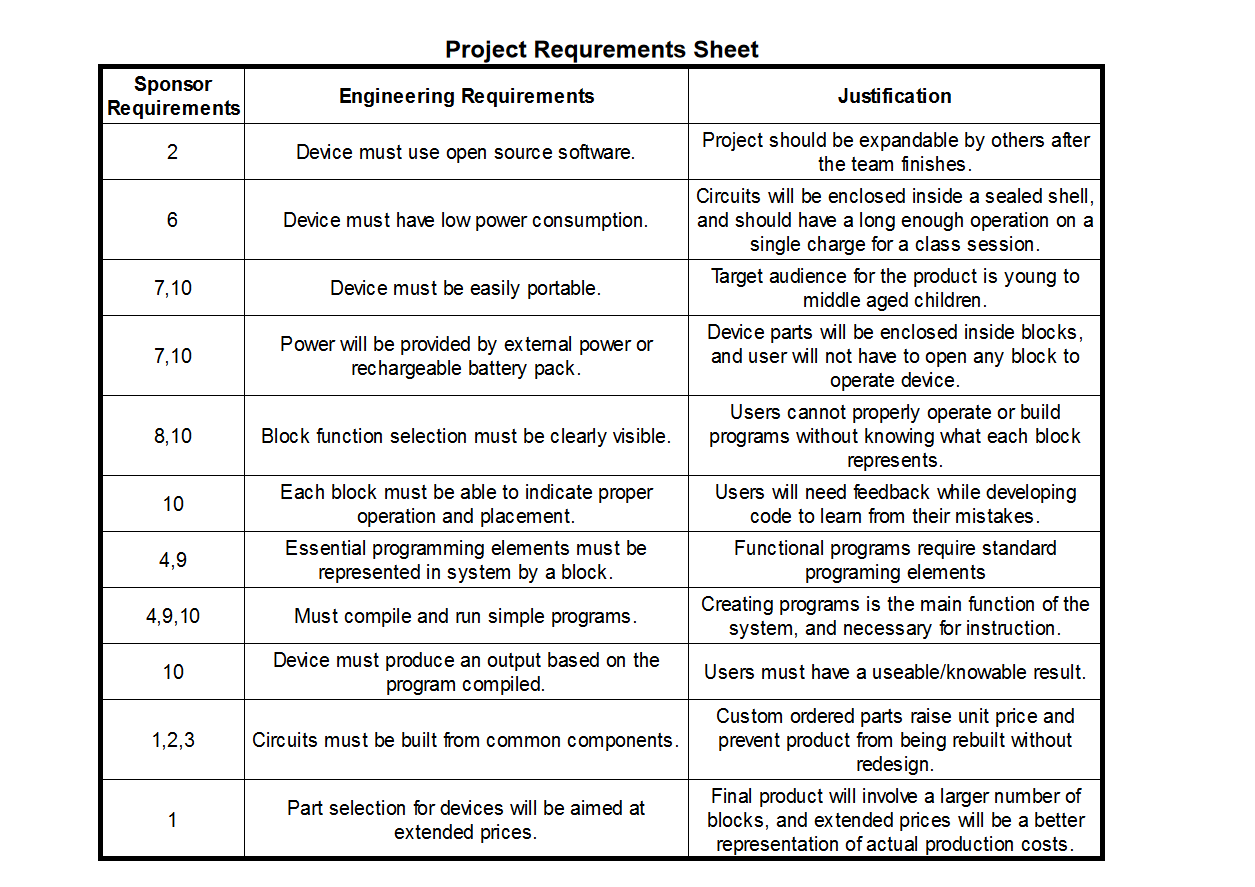
\includegraphics[width=6.5in]{pds.png}\\
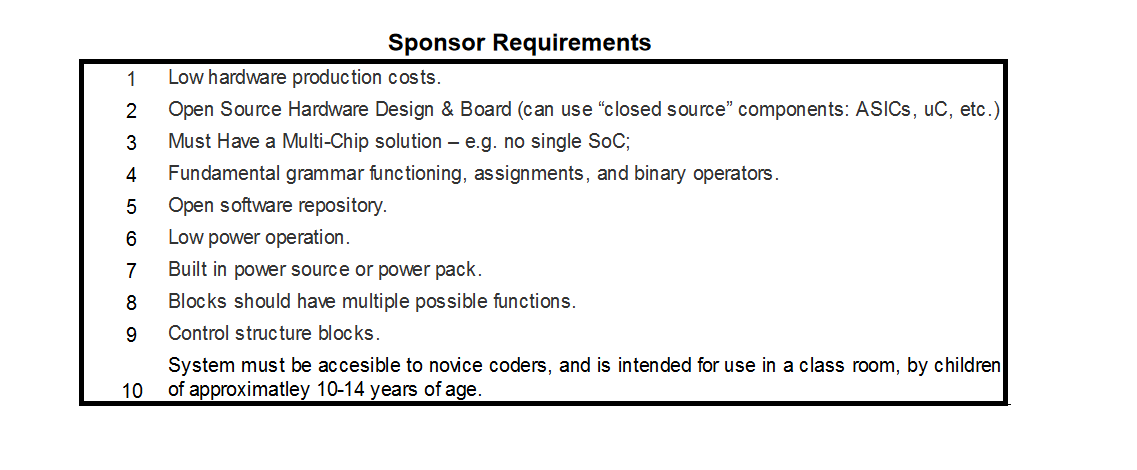
\includegraphics[width=6.5in]{sprq.png}
\section{Project Planning}
We identified three main elements for our system design: Physical Construction, Block Communication, and Program Interpretation. This enabled us to research and develop each subsystem in parallel with regular inter-group updates to stay unified on task. We also set several early milestones to ensure successful integration and to allow for multiple, iterative design revisions.

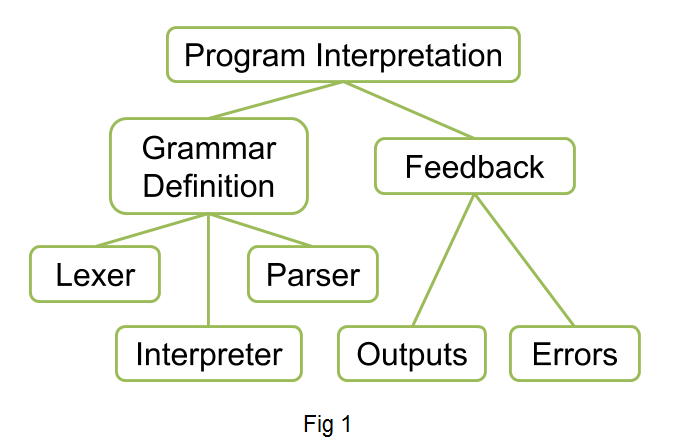
\includegraphics[width=4.25in]{PI.png}\\
\newpage
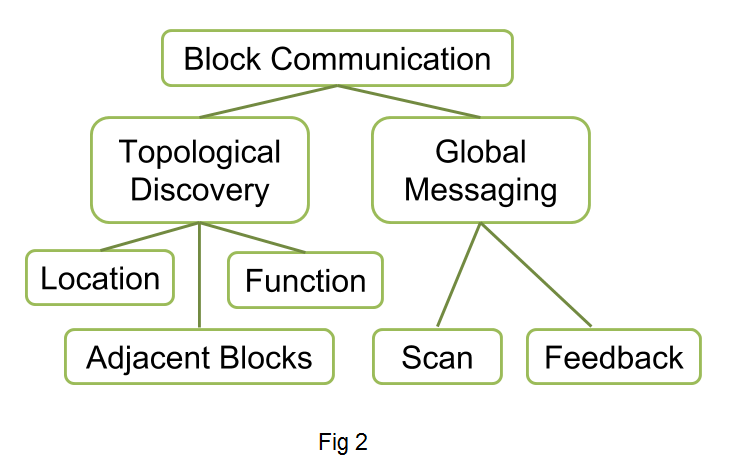
\includegraphics[width=4.75in]{BC.png}\\

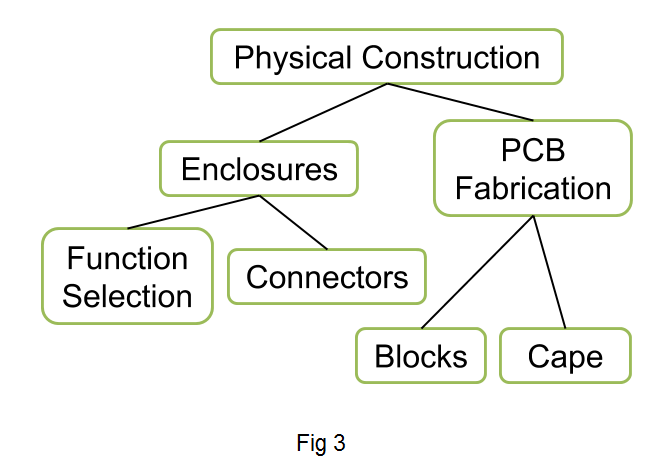
\includegraphics[width=4.75in]{PC.png}\\

With these divisions the work was scheduled based on skill, interest and load leveling.

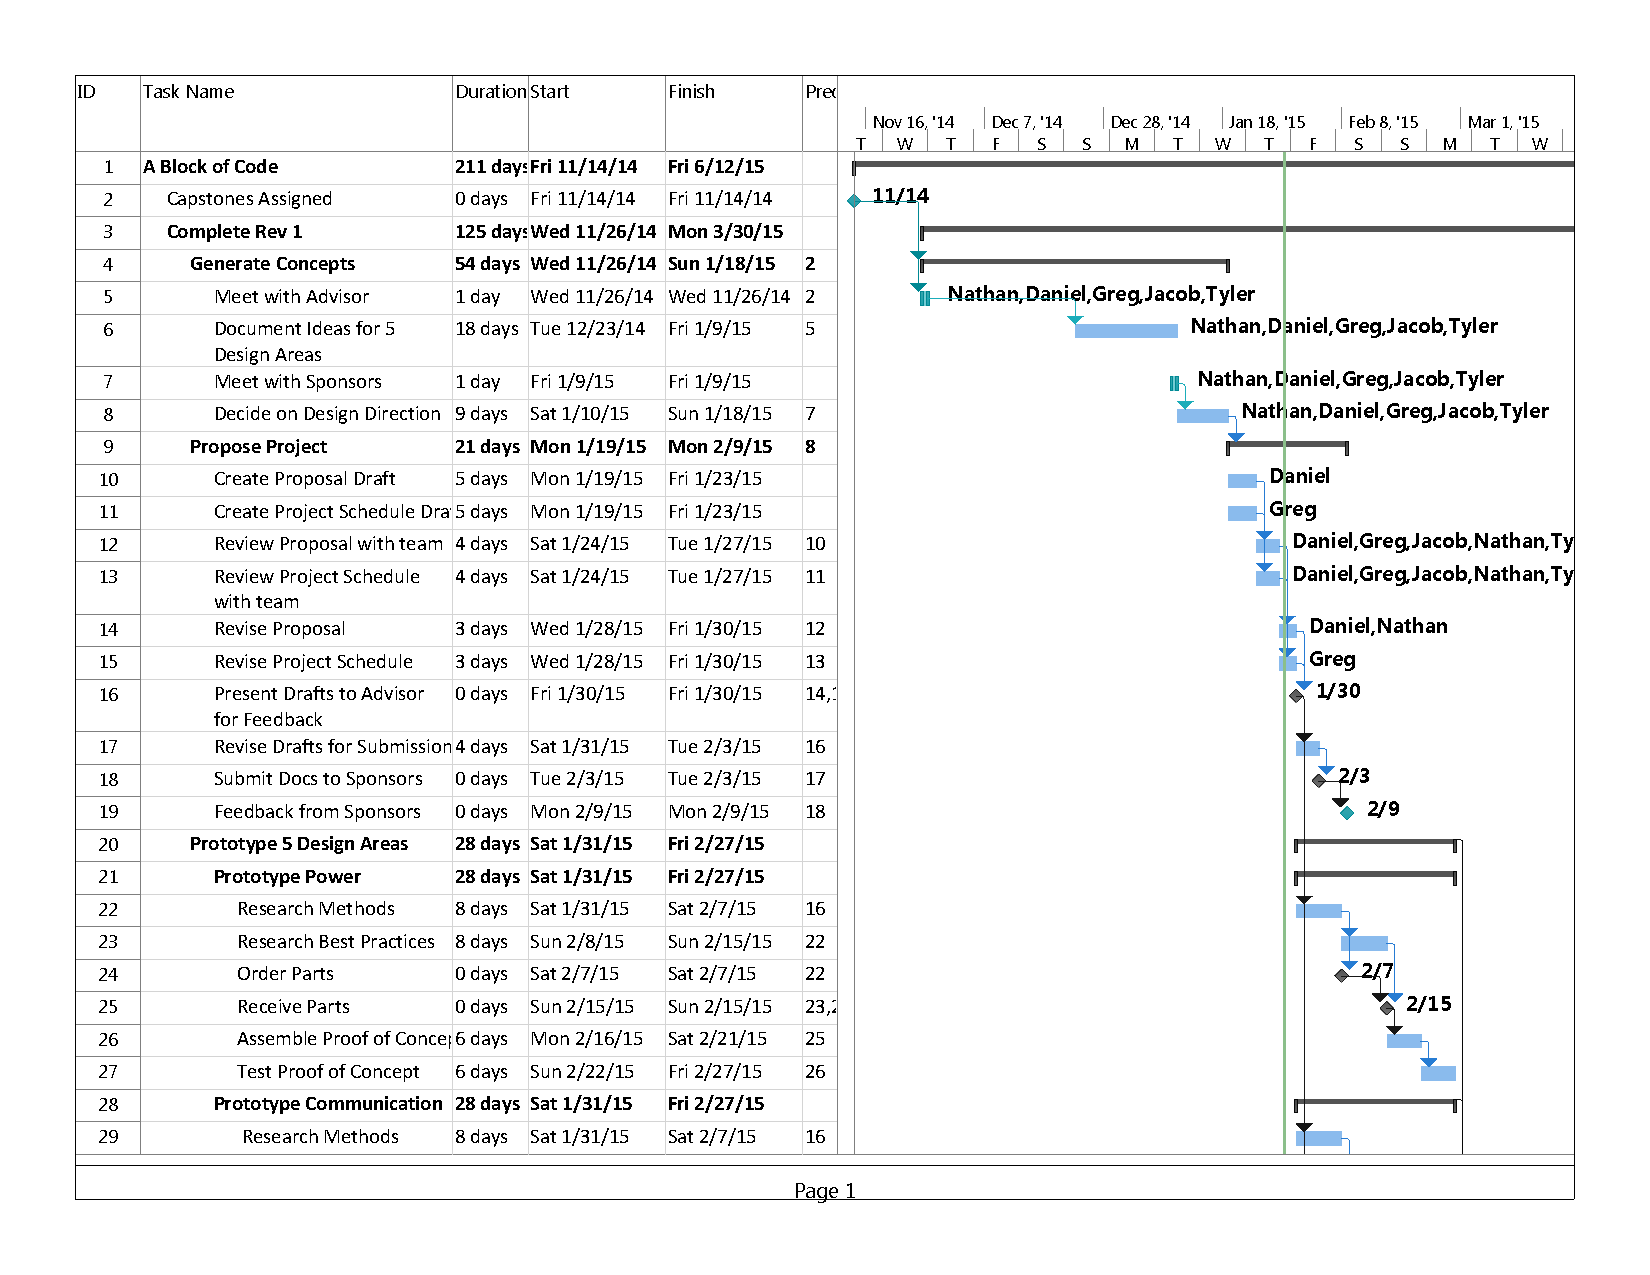
\includepdf[pages={1-}]{shed.pdf}
\section{Methods and Tools}
We utilized several methods and tools during all phases of the project, and some were used only for specific phases. We each used a mix of Windows, Macintosh, and Linux workstations throughout the project. We also used the AVR Toolchains (CrossPack, avr-gcc, avrdude) and the AVRISP MKII programmer in development, manufacturing, and testing. The BeagleBone Black was another major part of our full project cycle.

For our development phase, we utilized EagleCAD to design and layout prototype PCBs. We then moved to DesignSpark to allow us to develop 4-layer boards and reduce the surface area for a cheaper design. We employed an Arduino Uno and associated IDE to develop the TWI bus, initially with the smaller but compatible ATtiny85. We also used an Intronix Logicport 34-Channel Logic Analyzer to inspect communications, albeit much later in the process than necessary. We used a 3D printer to prototype a potential selector wheel.

During our manufacturing phase, we used the Portland State University Laboratory for Interconnected Devices to assemble both revisions of our prototype. We used their Torch T200N Reflow Oven to solder our second revision surface mount components. And we used their Full Spectrum Professional Series CO2 20x12 Laser to cut acrylic enclosures and selector wheels. We also used a handful of other Portland State tools such as soldering irons and a dremel. 

To test our final boards, we used a microscope to inspect solder connections and then a general purpose multimeter to verify conductivity and isolation. We then used an Arduino Uno?s regulated 3.3V output to supply power to a single and then a subset of blocks to confirm connectivity. We also wrote several scripts and test programs to explore the bounds and verify functionality of our set using an Arduino, a BeagleBone Black, and the blocks themselves.
\section{Implementation}
Our first development goal was a set of blocks that could identify their topology and return their token to a main processor. Though a ?smart-mat? design was considered, we decided it would be too dimensionally restrictive. We chose AVR microcontrollers and DB-9 connectors for their ease and cost. We utilized a localized SPI communication to establish location and a global TWI bus to report the block?s assigned value. We then selected a Linux-based single board computer to harness existing language parsing and interpretation tools. The BeagleBone Black provided this at reduced power.


Our second set of development goals aimed to the increase block-set capability, provide portability, and expand the available output options:
\begin{itemize}
	\item User-selectable subset of functions rather than a single, hard-coded token
	\item BeagleBone Controller Cape for power distribution and control of a global reset
	\item Additional modes of output connected to the Controller Cape to support student engagement in learning programming concepts
	
\end{itemize}
ach block is controlled by an ATtiny461 microcontroller, connected to two neighbors on a local bus based on SPI, and connected to all other blocks and the BeagleBone Black on a global bus using TWI. Both of these busses, as well as power and ground, are brought onto the block via a standard DB-9 connector. The token selector wheel is mounted on a 1 M? potentiometer which feeds into the ADC on the microcontroller.


The local bus is started from the BeagleBone and initiates a handshake with the block connected below it. When the handshake completes, a vector is passed indicating the x- and y-coordinates of the sending block. The receiving block increments the vector based on whether the sending block is signaling from the above or the left line of the receiving block, and then stores and sends the incremented vector to the next block. The received vector is then translated into the TWI address on the global bus. The BeagleBone Black is able to query each block which responds with information on its adjacent blocks, its wheel category, and its current ADC value. The BeagleBone Black lexer uses this response data to construct a topology of the current block arrangement. It then passes this information to a parser and interpreter to generate the appropriate output such as driving a LCD screen.
\subsection{Block}
    The primary function of each block is to report back to the main processor board its own user-selected function as well as its adjacent blocks. This allows the main processor to collect the tokens and topological information necessary for constructing the user-generated program. A block progresses linearly through a series of states as outlined in the state diagram, Fig 4, on the following page.
  \subsubsection{Adjacent Blocks}  
  First, the block will execute an initialization sequence that includes outputting to and reading from its adjacency lines. In typical usage, the blocks are built in a top-down orientation. A pair of slave-select pins, connected to the right and bottom connectors, are designated as temporarily as inputs with their internal pull-up resistors enabled. Another pair of slave-select pins, connected to the left and top connectors, are designated temporarily as outputs and immediately pulled low. 
  
  For an example, consider the top block in Fig 5. If the block reads its adjacency pins and finds that its h\_out line (horizontal output) is HIGH, then it has no block connected to its right (again, in a top-down orientation). If it reads its v\_in is LOW, then a block is present below it. These values are stored and supplied to the main processor board in a global bus response (see TWI Commands).
  
    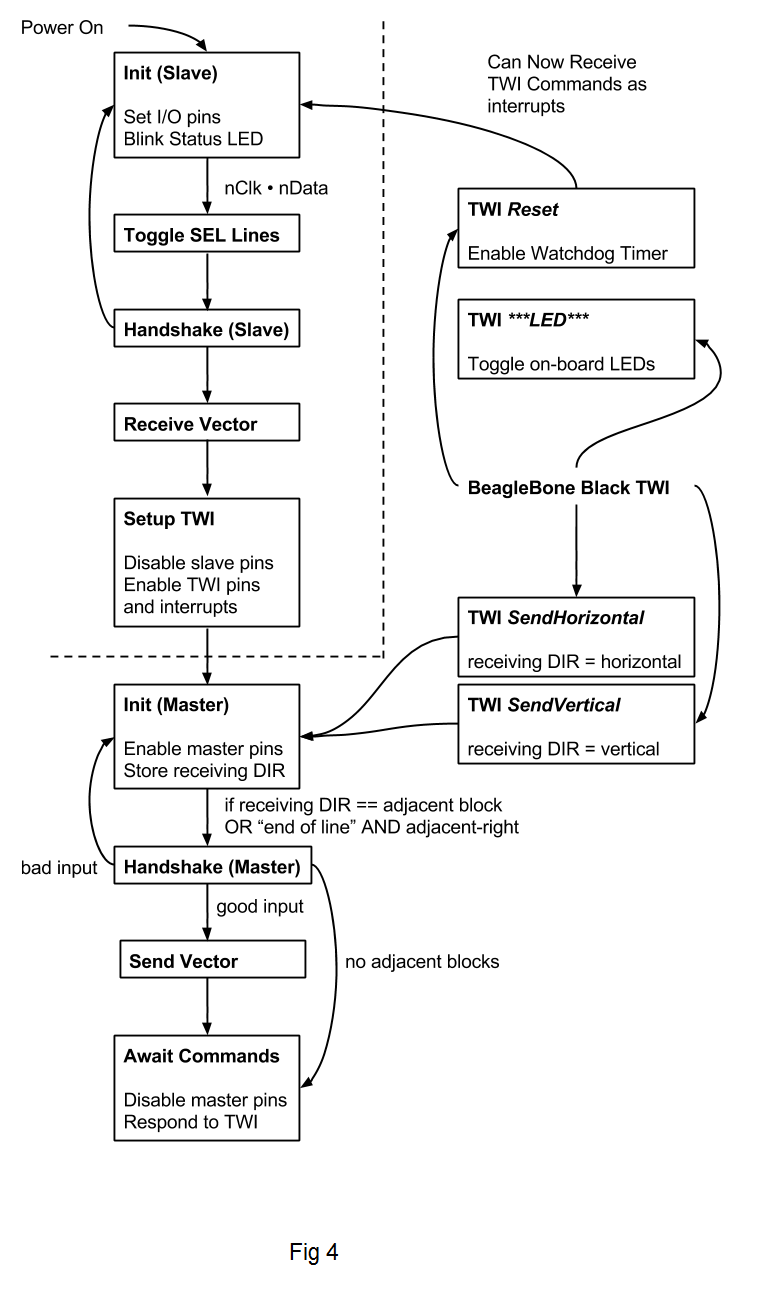
\includegraphics[width=4.75in]{USD.png}\\
    
 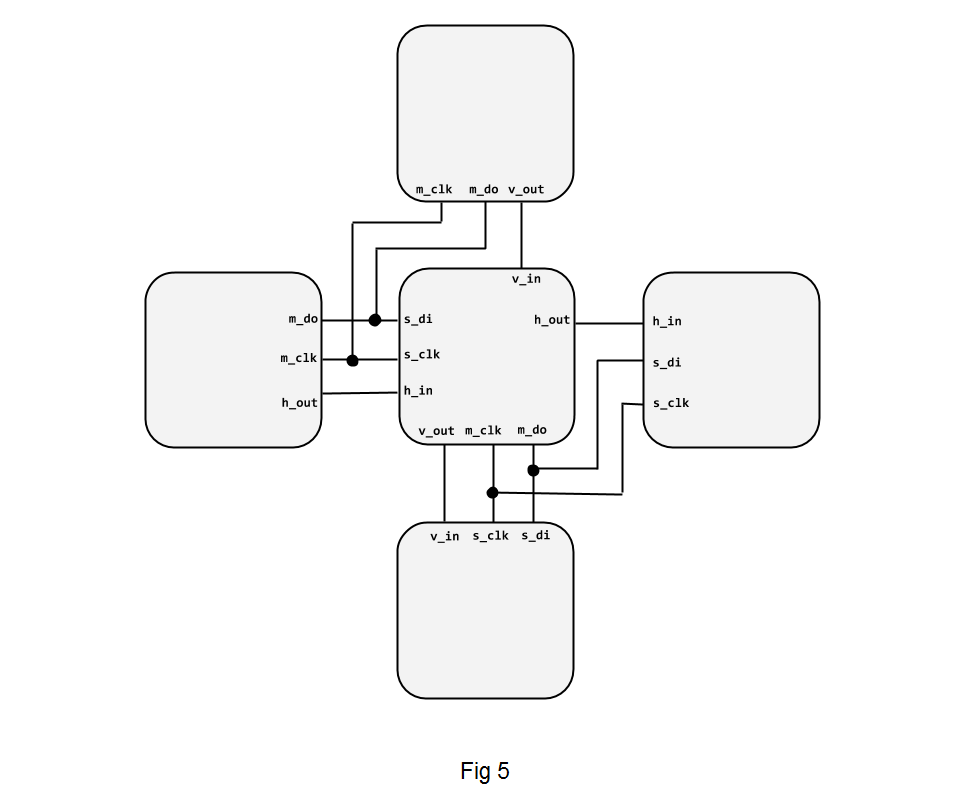
\includegraphics[width=4.25in]{BD.png}
 \subsubsection{Handshake}
 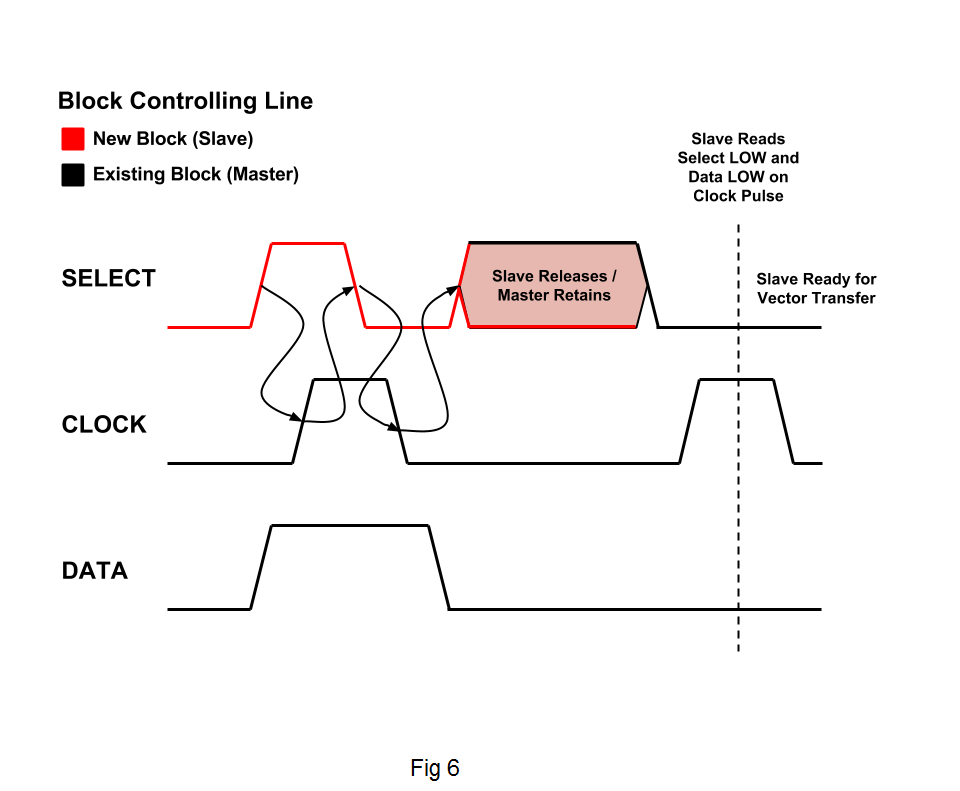
\includegraphics[width=4.5in]{HS.png}
 After the a block is powered on and has executed its initialization sequence, including determining adjacent blocks, it prepares for a custom handshake to initiate a SPI transmission. Shown above is this handshake, where the just-powered-on block is considered the slave, and another block or the BeagleBone Black is considered the master. 
 
 \begin{enumerate}
 	\item First, the block will wait for the shared clock and data lines to go LOW. This will signal the block to start toggling its own select lines (v\_in and h\_in). 
 	\item The master will then respond to the toggle that it sees (either horizontally or vertically) by bringing clock and data HIGH. 
 	\item This triggers the select line LOW again and the clock and data lines again follow. 
 	\item Next, the slave block brings its select line HIGH yet again but then releases control of it by switching the pin to an input and enable its internal pull-up resistor. 
 	\item The master waits a short delay after seeing that rising edge then it changes its corresponding select line from an input to an output and pulls the line LOW. 
 	\item A final clock pulse acts as a verification of the completed sequence before both blocks are prepared for a traditional SPI transmission.
 \end{enumerate}
 
 It is possible that an adjacent block could see the same clock and data lines go LOW and in fact complete almost the entire sequence. But the corresponding select line would not be held low on that final clock pulse and thus that block would recognize that the sequence was not meant for it, and reset its state. The same is true for any other sequence of edges that doesn't follow here -- it would be considered bad input and cause a reset to initial handshake state.
 \subsubsection{SPI Transmission}
 Once a block has completed its handshake, it is prepared to receive data over a three-wire SPI protocol. This means there is no MISO signal involved. After the data is received, the block is able to continue to send the data to adjacent blocks as necessary. It will continue the direction it was originally sent (e.g. if received from above, send below; if received from the left, send right). 
 
 
 It will also recognize when it is considered the ?end of the line,? which is considered the block with x-coordinate of 0 and no blocks connected below it. In this special case, it will then send to the right if there is a block present. 
 Finally, a block will send in the vertical or horizontal directions on command from the global TWI bus (see TWI Commands). 
 
 
 Below is a screen capture from a logic analyzer showing 3 different SPI transmissions (in this example, blocks are implemented in a bottom-up orientation). The first transmission is to the current block which is acting as a slave and receiving data. The handshake begins at about the -200ms mark and completes roughly at -135ms mark. The actual transfer is shortly after that. The second handshake begins immediately and two lines do in fact follow the sequence, but only one has its line low when a second clock pulse ?confirms? the exchange. Finally, a TWI command is issued at about the -10ms mark to complete that last SPI transmission.\\
 
 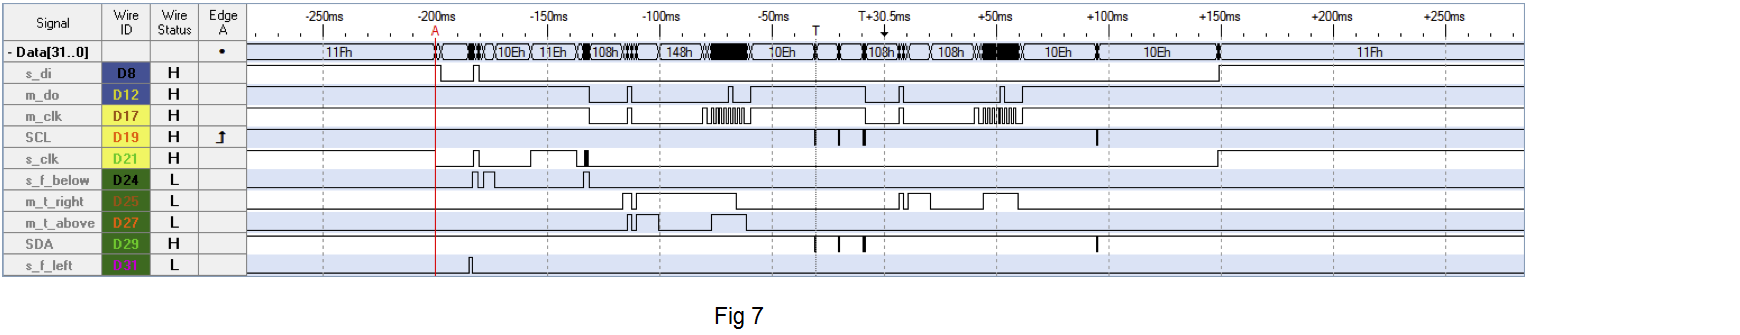
\includegraphics[width=7in]{RCC.png}
  The data transferred is an encoded vector indicated the sending-block?s coordinates in the xy-plane of the user-program?s topology: the first 3 bits are the x-coordinate, and the next 4 bits are the y-coordinate. The receiving block will add 1 to the x- or y-coordinate it received, depending on from which direction it was sent. If an overflow will occur (e.g. if the block receives a x-coordinate of 7 from the left, it would increment to 8 which would overflow beyond the allotted 3 bits), then the process is aborted and an error indicating LED will blink to indicate the error condition. Otherwise, this encoded and incremented vector becomes the address of this block for a Two-Wire Interface global bus.
  
  \subsubsection{TWI Commands}
  The TWI interface allows targeted commands to trigger a handful of actions. The BeagleBone Black issues a TWI read request indicating an address (block) and a register (command). These numbers act as virtual registers on the block and are captured to issue tasks in a work queue. Below is a table of all the implemented actions. 
  
  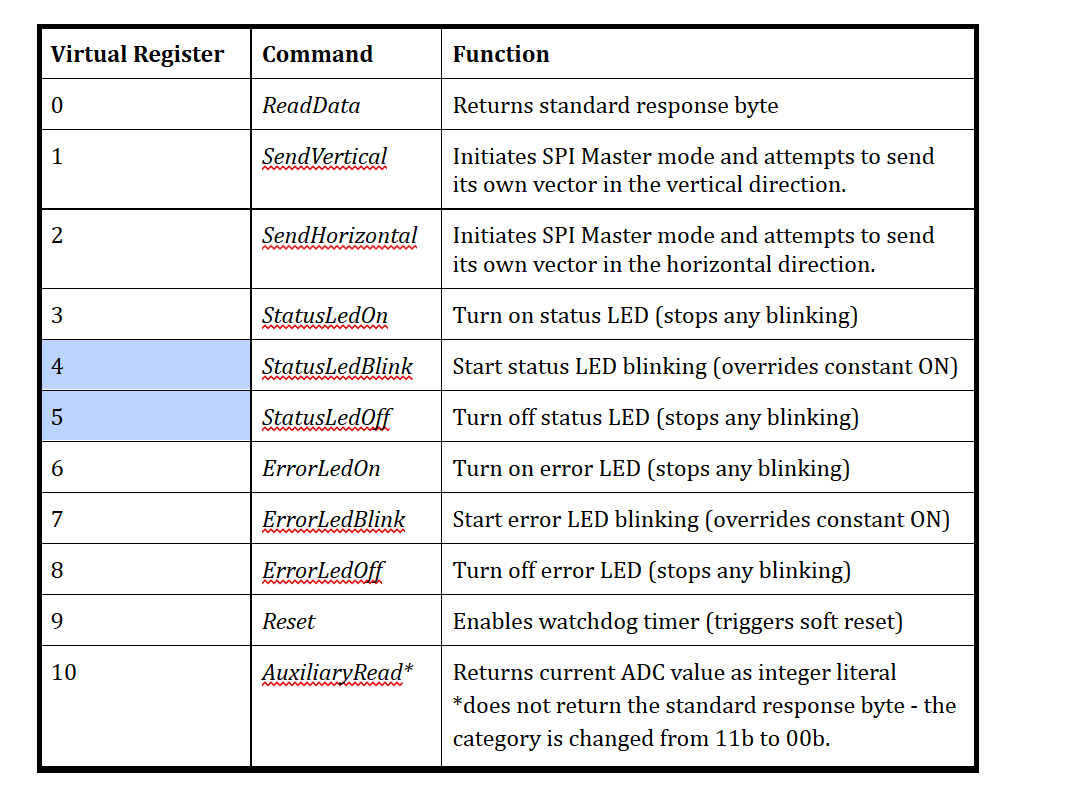
\includegraphics[width=6.5in]{vrc.png}
  Each command (except for number 10) returns a response byte that shows the current status of the addressed block. This byte is described below:
    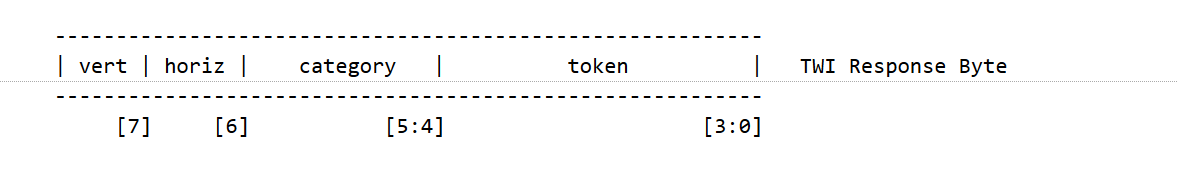
\includegraphics[width=6.5in]{TWI.png}
    
    \newpage
    The most significant two bits are flags indicating if the current block has adjacent blocks connected in the vertical and horizontal directions respectively. The next two bits identify the category (or wheel) that is used for this block. And finally, the remaining four bits are the most significant 4 bits from the ADC read from the potentiometer. This indicates the user-selected token and, combined with the category identifier, indicates the exact token to be used in the parser. 
    
    \subsection{Processor Board}
    \subsubsection{Lexer}
    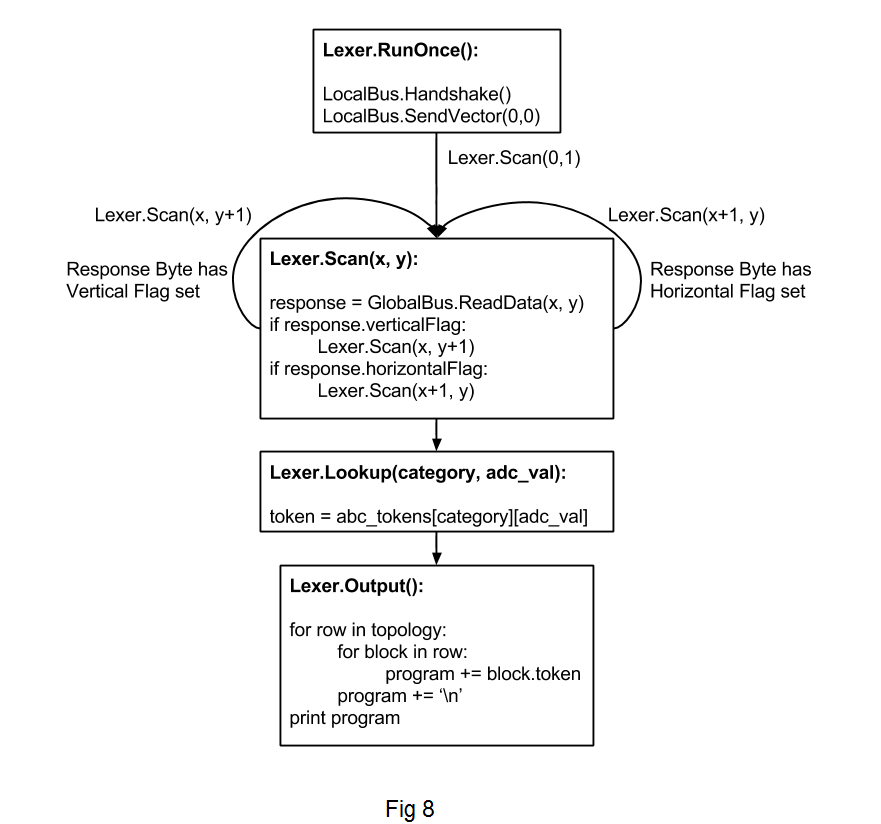
\includegraphics[width=4.5in]{LX.png}
    The lexer on the BeagleBone Black utilizes both the local SPI-based bus as well as the global TWI-based bus. The BeagleBone Black initiates a standard handshake, as described above, and sends its own coordinate of (0, 0) to the connected block. This starts a chain of sending vectors to the ?end of the line.? The lexer then uses the TWI to query the first block with a ReadData command, and recursively traverses the topology according to the vertical and horizontal adjacency flags in the response byte. 
    
    
    For each block response it receives with the vertical flag set, it queries the next vertical address until it receives a response without that flag set. It then sends a SendHorizontal command to the next block with a x-coordinate of zero and a horizontal adjacency flag set. The lexer queries that row until it gets to the end and then sends the next SendHorizontal command as necessary. This collects all the blocks (including their categories and ADC values). Each block?s ADC value and category is used as keys to a master token lookup table, shown in the table on the following page.     The lexer then prints a string constructed from the mapped tokens to stdout which is captured by the parser / interpreter.
    
    
     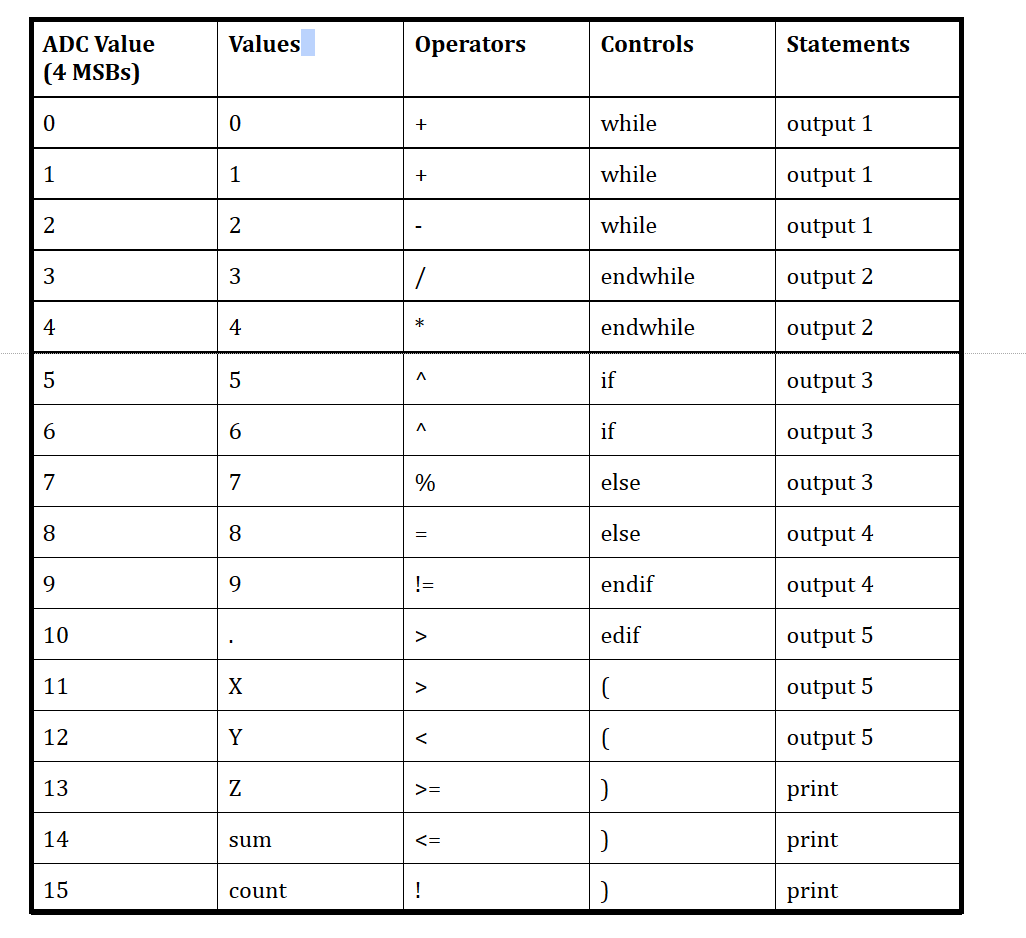
\includegraphics[width=6.5in]{lxer.png}
\end{document}
